\documentclass{beamer}

%
% Choose how your presentation looks.
%
% For more themes, color themes and font themes, see:
% http://deic.uab.es/~iblanes/beamer_gallery/index_by_theme.html
%
\mode<presentation>
{
  \usetheme{Madrid}      % or try Darmstadt, Madrid, Warsaw, ...
  \usecolortheme{beaver} % or try albatross, beaver, crane, ...
  \usefonttheme{serif}  % or try serif, structurebold, ...
  \setbeamertemplate{navigation symbols}{}
  \setbeamertemplate{caption}[numbered]
} 

% packages
\usepackage[english]{babel}
\usepackage[utf8]{inputenc}
\usepackage[T1]{fontenc}
\usepackage{graphicx}
\usepackage{wrapfig}
\usepackage{amsmath, amssymb}


%tikz
\usepackage{tikz}
\usetikzlibrary{shapes,snakes,arrows, chains, positioning, shapes.geometric, shapes.symbols,calc,shadows}
\usepackage{tikz-3dplot}
\tdplotsetmaincoords{70}{110}
\usepackage{tikz-cd}
\def\centerarc[#1](#2)(#3:#4:#5)% Syntax: [draw options] (center) (initial angle:final angle:radius)
{ \draw[#1] ($(#2)+({#5*cos(#3)},{#5*sin(#3)})$) arc (#3:#4:#5); }

% commands
\newcommand{\C}{\mathbb{C}}
\newcommand{\Q}{\mathbb{Q}}
\newcommand{\R}{\mathbb{R}}
\newcommand{\Z}{\mathbb{Z}}
\renewcommand{\P}{\mathbb{P}}
\newcommand{\CP}{\mathbb{CP}}

\newcommand{\mA}{\mathcal{A}}
\newcommand{\mB}{\mathcal{B}}
\newcommand{\mC}{\mathcal{C}}
\newcommand{\mE}{\mathcal{E}}
\newcommand{\mF}{\mathcal{F}}
\newcommand{\mG}{\mathcal{G}}
\newcommand{\mK}{\mathcal{K}}
\newcommand{\mO}{\mathcal{O}}
\newcommand{\mH}{\mathcal{H}}
\newcommand{\mI}{\mathcal{I}}
\newcommand{\mT}{\mathcal{T}}
\newcommand{\mL}{\mathcal{L}}
\newcommand{\mN}{\mathcal{N}}
\newcommand{\mP}{\mathcal{P}}
\newcommand{\mQ}{\mathcal{Q}}
\newcommand{\mS}{\mathcal{S}}
\newcommand{\mU}{\mathcal{U}}
\newcommand{\mV}{\mathcal{V}}

\newcommand{\ba}{\mathbf{a}}
\newcommand{\bb}{\mathbf{b}}
\newcommand{\be}{\mathbf{e}}
\newcommand{\bF}{\mathbf{F}}
\newcommand{\bx}{\mathbf{x}}

\newcommand{\mLi}{\mathcal{L}_{\textup{irr}}}
\newcommand{\mLr}{\mathcal{L}_{\textup{red}}}
\newcommand{\p}{\partial}
\newcommand{\iprod}{\mathbin{\lrcorner} \,}

\newcommand{\tL}{\widetilde{L}}
\newcommand{\tM}{\widetilde{M}}
\newcommand{\tH}{\widetilde{H}}
\newcommand{\tmH}{\widetilde{\mH}}
\newcommand{\tx}{\widetilde{x}}
\newcommand{\tp}{\widetilde{p}}
\newcommand{\tX}{\widetilde{X}}
\newcommand{\tD}{\widetilde{D}}
\newcommand{\tY}{\widetilde{Y}}
\newcommand{\tN}{\widetilde{N}}
\newcommand{\tP}{\widetilde{P}}
\newcommand{\tQ}{\widetilde{Q}}
\newcommand{\tV}{\widetilde{V}}
\newcommand{\newpar}{\vspace{0.15in}}

\newcommand{\tv}{\tilde{v}}

\newcommand{\txA}{\textup{A}}
\newcommand{\txB}{\textup{B}}
\newcommand{\txC}{\textup{C}}

\newcommand{\rI}{\mathring{I}}

\newcommand{\hL}{\widehat{L}}
\newcommand{\hH}{\widehat{H}}
\newcommand{\hx}{\widehat{x}}
\newcommand{\hX}{\widehat{X}}

\newcommand{\bc}{\mathbf{c}}
\newcommand{\bv}{\mathbf{v}}

\DeclareMathOperator{\rk}{rank}
\DeclareMathOperator{\spn}{span}
\DeclareMathOperator{\codim}{codim}
\DeclareMathOperator{\parch}{par-ch}
\DeclareMathOperator{\parc}{par-c}
\DeclareMathOperator{\pardeg}{par-deg}
\DeclareMathOperator{\ch}{ch}
\DeclareMathOperator{\Hom}{Hom}
\DeclareMathOperator{\Gr}{Gr}
\DeclareMathOperator{\Aut}{Aut}
\DeclareMathOperator{\Pic}{Pic}
\DeclareMathOperator{\Bl}{Bl}
\DeclareMathOperator{\Res}{Res}
\DeclareMathOperator{\End}{End}
\DeclareMathOperator{\tr}{tr}
\DeclareMathOperator{\diag}{diag}
\DeclareMathOperator{\pr}{pr}
\DeclareMathOperator{\vol}{vol}
\DeclareMathOperator{\CY}{CY}
\DeclareMathOperator{\etop}{top}
\DeclareMathOperator{\orb}{orb}
\DeclareMathOperator{\Sing}{Sing}
\DeclareMathOperator{\PGL}{PGL}
\DeclareMathOperator{\Tan}{Tan}
\DeclareMathOperator{\Irr}{Irr}
\DeclareMathOperator{\wt}{wt}
\DeclareMathOperator{\im}{im}
\DeclareMathOperator{\Ric}{Ric}
\DeclareMathOperator{\Cl}{Cl}
\DeclareMathOperator{\loc}{loc}
\DeclareMathOperator{\FS}{FS}
\DeclareMathOperator{\RF}{RF}
\DeclareMathOperator{\KE}{KE}
\DeclareMathOperator{\Stab}{Stab}
\DeclareMathOperator{\PG}{PG}
\DeclareMathOperator{\Id}{Id}

%commands
\newcommand{\mathcolorbox}[2]{\colorbox{#1}{$\displaystyle #2$}}

%\DeclareMathOperator{\tr}{tr}

%\DeclareMathOperator{\codim}{codim}

% openning
\title[]{Miyaoka-Yau inequality for hyperplane arrangements}
\author[Integrable Day]{Martin de Borbon}
\addtobeamertemplate{author}{}{arXiv: 2411.09573 (joint with Dmitri Panov)}
\institute[Loughborough]{Loughborough University}
\date{}

\begin{document}

\begin{frame}
  \titlepage
\end{frame}

% Uncomment these lines for an automatically generated outline.
%\begin{frame}{Outline}
%  \tableofcontents
%\end{frame}

\section{Introduction}

\begin{frame}{Plan}
	\begin{itemize}
		\item Main result
		\vfill
		\item Proof
		\vfill
		\item Application
	\end{itemize}
\end{frame}

\begin{frame}{Basic definitions}
	\begin{itemize}
		\item This is a paper about complex projective space
		\begin{equation*}
			\CP^n = \left(\C^{n+1} \setminus \{0\}\right) \big/ \, \C^*	\,.
		\end{equation*} 
		\vfill
		
		\item Let \(\mH\) be a hyperplane arrangement in \(\CP^n\).
		That is, \(\mH\) is a finite set of pairwise distinct complex hyperplanes 
		\[
		H \subset \CP^n \,.
		\]
		\vfill
		
		\item Let \(L \subset \CP^n\) be a linear subspace  obtained as intersection of hyperplanes \(H \in \mH\). 
		The \textbf{multiplicity} of \(L\) is
		\[
		m_L = \big| \{H \in \mH \,|\, H \supset L\} \big| \,.
		\]
	\end{itemize}
	
\emph{Note:} \(m_L \geq \codim L\)
\end{frame}


\begin{frame}{Codimension \(2\) subspaces}
	Let \(L \subset \CP^n\) be a codimension \(2\) intersection of hyperplanes in \(\mH\). 
	
	We say that
	\begin{itemize}
		\item \(L\) is \textbf{reducible} if \(m_L = 2\)
		\item \(L\) is \textbf{irreducible} if \(m_L \geq 3\)
	\end{itemize}
	
	\begin{figure}[h]
		\centering
			\begin{minipage}{0.48\textwidth}
				\scalebox{0.6}{
					\begin{tikzpicture}[tdplot_main_coords,font=\sffamily]
						\draw[fill=blue,opacity=0.2] (-3,0,-3) -- (-3,0,3) -- (3,0,3) -- (3,0,-3) -- cycle;
						\draw[fill=blue,opacity=0.2] (0,-3,-3) -- (0,-3,3) -- (0,3,3) -- (0,3,-3) -- cycle;
											
						\draw[thick] (0,0,-3)--(0,0,3);
						\node[scale=1.5] at (0,.3) {\(L\)};		
					\end{tikzpicture}
				}
			\end{minipage}	
			\begin{minipage}{0.48\textwidth}
				\scalebox{0.6}{
					\begin{tikzpicture}[tdplot_main_coords,font=\sffamily]
						\draw[fill=blue,opacity=0.2] (-3,0,-3) -- (-3,0,3) -- (3,0,3) -- (3,0,-3) -- cycle;
						\draw[fill=blue,opacity=0.2] (0,-3,-3) -- (0,-3,3) -- (0,3,3) -- (0,3,-3) -- cycle;
						\draw[fill=blue,opacity=0.2] (-3,-3,-3) -- (3,3,-3) -- (3,3,3) -- (-3,-3,3) -- cycle;
						
						\draw[thick] (0,0,-3) -- (0,0,3);
						\node[scale=1.5] at (0,.3) {\(L\)};
					\end{tikzpicture}
				}
			\end{minipage}	
		\caption{Reducible (left) and irreducible (right).}
		\label{fig:codim2}
	\end{figure}
\end{frame}

\begin{frame}{The Hirzebruch quadratic form}
	\begin{itemize}
		\item \(\mH = \{H_1, \ldots, H_N\}\) hyperplane arrangement in \(\CP^n\)
		\item \(\sigma_i = \) number of irreducible codimension \(2\) subspaces \(L \subset H_i\)
		\item The \textbf{Hirzebruch quadratic form} of \(\mH\) is the homogeneous degree \(2\) polynomial on \(\R^N\) given by
	\end{itemize}
	\[
	Q(a_1, \ldots, a_N) = \sum_{i,j = 1}^N Q_{ij} a_i a_j 
	\]
	\[
	\mathcolorbox{green!20}{
	Q_{ij} = \begin{cases}
		- (n+1) \sigma_i + 2n &\text{ if } i = j  \\
		-2 &\text{ if }  i \neq j \text{ and } L = H_i \cap H_j \text{ is reducible} \\
		\,\, n-1 &\text{ if } i \neq j \text{ and } L = H_i \cap H_j \text{ is irreducible} 
	\end{cases}
}
	\]
\end{frame}

\begin{frame}{H\"ofer's formula}
	\begin{center}
		\begin{figure}
			\includegraphics[width=0.8\textwidth,height=0.8\textheight,keepaspectratio]{hofer}
		\end{figure}
	\end{center}
\end{frame}

\begin{frame}{The matroid polytope}
	\(\mH\) is an \emph{essential} and \emph{irreducible} hyperplane arrangement in \(\CP^n\)
	\vfill
	\begin{itemize}	
		\item A \textbf{basis} of \(\mH = \{H_1, \ldots, H_N\}\) is a subset \(\mB \subset \mH\) consisting of \(n+1\) linearly independent hyperplanes
		\vfill
		\item The indicator vector of \(\mB\) is the 1/0 vector
		\[
		\be_{\mB} = \sum_{i \,|\, H_i \in \mB} \be_i
		\]
		where \(\be_1, \ldots, \be_N\) are the standard basis vectors of \(\R^N\)
		\vfill
		\item The \textbf{matroid polytope} is the convex hull of the vectors \(\be_{\mB}\)
		\[
		P = \mathrm{conv} \{\, \be_{\mB} \,\,|\,\, \mB \, \text{ is a basis of } \mH \,\} \,.
		\]
	\end{itemize}
	Note: \(P\) is contained in the \((N-1)\)-simplex \(\Delta \subset \R^N\) with
	\[
	\Delta = \big\{\, (a_1, \ldots, a_N) \in \R^N \,|\, a_i \geq 0, \,\, \sum_i a_i = n+1 \, \big\}
	\]
\end{frame}

\begin{frame}{The semistable and stable cones}
	\begin{itemize}
		\item The \textbf{semistable cone} is the cone over the matroid polytope
		\[
		C = \R_{\geq 0} \cdot P = \mathrm{cone} \,\, \{\, \be_{\mB} \,\,|\,\, \mB \, \text{ is a basis of } \mH \,\} \,.
		\]
		It is a convex polyhedral cone contained in the octant \(\R^N_{\geq 0}\)
		\vfill
		
		\item The \textbf{stable cone} is the interior of \(C \subset \R^N\)
		\[
		C^{\circ} = \mathrm{int} (C) \,.
		\]
		\vfill
		
		\item \(\mH\) is essential and irreducible \(\iff\) \(\dim P = N-1\)
		
		\phantom{\(\mH\) is essential and irreducible} \(\iff\) \(C^{\circ}\) is non empty
	\end{itemize}
\end{frame}

\begin{frame}{Defining linear inequalities of \(C^{\circ}\)}
	\begin{itemize}
		\item Let \(\mL\) be the finite set of \emph{non-empty} and \emph{proper} linear subspaces \(L \subset \CP^n\) obtained by intersecting members of \(\mH\)
		
		\item \((a_1, \ldots, a_N) \in C^{\circ}\) \(\iff\) \(\forall i:\) \(a_i > 0\)  and \(\forall L \in \mL:\)
		\[
		\mathcolorbox{green!20}{
			\sum_{i \,|\, L \subset H_i} a_i < \frac{\codim L}{n+1} \cdot \sum_{i=1}^{N} a_i 
		}
		\]
		
	\end{itemize}
\end{frame}


\begin{frame}{Introduction}
	\begin{itemize}
		\item \textbf{Long term goal:} produce (and classify) constant holomorphic sectional curvature metrics with cone singularities using (singular, i.e. logarithmic) flat connections.
		
		\item \textbf{Precedents:} 
		\begin{itemize}
			\item Smooth case. Hitchin gave a proof of the Uniformization Theorem (existence of hyperbolic K\"ahler metrics on compact Riemann surfaces) using the theory of Higgs bundles. 
			
			Simpson extended the method to higher dimensions. In particular, he used Higgs bundles to prove the Miyaoka-Yau characterization of compact complex hyperbolic surfaces.
			
			\item Panov used the parabolic Kobayashi-Hitchin correspondence to classify \textbf{polyhedral K\"ahler} (PK) metrics on \(\CP^2\) with cone angles \(<2\pi\) along line arrangements.
		\end{itemize}
	
	\item \textbf{Key technical point:} analyse connections of the form
	\[ \mathcolorbox{blue!20}{
		\nabla = d - \sum_{H \in \mathcal{H}} A_H \frac{dh}{h} 
	}
	\]
	
	\end{itemize}
\end{frame}

\section{2-dim models}

\begin{frame}{\(2\)-dim models}
	Fix \(\mathcolorbox{blue!20}{\alpha>0}\). The models
	\[
	\begin{cases}
	dr^2 + \alpha^2 (\sin^2r) d\theta^2 \\
	dr^2 + \alpha^2 r^2 d\theta^2 \\
	dr^2 + \alpha^2 (\sinh^2r) d\theta^2 	
	\end{cases}
	\]
	define constant curvature metrics with cone angle \(2\pi\alpha\) at the origin.
	
	\textbf{Examples.}
	
	\begin{itemize}
		\item Orbifold quotients \(\alpha=1/k\), pull-backs \(\alpha=k\)
		\item Doubles of (spherical/Euclidean/hyperbolic) polygons
		\item Polyhedral (spherical/Euclidean/hyperbolic) surfaces
	\end{itemize}
\end{frame}

\section{Unif}

\begin{frame}{Uniformization}
	\(S\) compact oriented surface with cone points \(2\pi\alpha_1, \ldots, 2\pi\alpha_N\)
	\begin{itemize}
		\item Gauss-Bonnet: \(\mathcolorbox{yellow!40}{a_i = 1-\alpha_i}\)
		\[\frac{1}{2\pi}\int_S K dA = \chi(S) - \sum_i a_i \]
		\item Anti-clockwise rotation by \(90^{\circ}\) gives a smooth complex structure
		\[ \{ \text{const. curv., angles } 2\pi\alpha_i \} \xrightarrow{\Phi} \{ \text{pairs } (X, \sum_i a_i \cdot x_i) \} \]
		Quotient by isometries/scale and marked bihol. 
	\end{itemize}
	
	\begin{theorem}[McOwen, Troyanov, Luo-Tian, ...]
		\(\Phi\) defines a bijection if \(\chi(S, \alpha) \leq 0\) or \(\chi(S, \alpha)>0\) where: \(0< \alpha_i < 1 \hspace{1mm} \mathrm{(so} \hspace{1mm} X\cong \CP^1 \mathrm{)}\) and \(a_i < \sum_{j\neq i} a_j \) with \(N \geq 3\)
	
	\end{theorem}
\end{frame}

\section{Sph. triang.}

\begin{frame}{Example: spherical triangles}
	Let \(T\) be a spherical triangle with interior angles \(\pi\alpha_i\) with \(0<\alpha_i<1\) 
	\[\mbox{area}(T) = \pi (\alpha_1+\alpha_2+\alpha_3-1)
	\]
	\(T\) is the intersection of \(3\) spherical wedges \(W_i\) with
	\[\mbox{area} (W_i) = 2\pi \alpha_i
	\]
	The inequalities \(\mbox{area}(T)>0\) together with \(\mbox{area}(T)<\mbox{area}(W_i)\) define a simplex inside the unit cube \(Q=\{0<\alpha_i<1\}\) given by
	\[\sum_i a_i < 2, \hspace{2mm} a_i < a_j + a_k
	\]
	Reflecting the simplex across the faces of \(Q\) and it translates gives all possible spherical triangles with arbitrary large (non-integer) angles
	
	
\end{frame}


\section{PK cones C2}
\begin{frame}{PK cone metrics on \(\C^2\)}

\begin{center}
	\scalebox{.6}{
		\begin{tikzpicture}
		%circles
		\centerarc[red](0,0)(57:110:1);
		\centerarc[red](0,0)(115:410:1);
		\centerarc[blue](1.2,0)(-124:65:1);
		\centerarc[blue](1.2,0)(70:230:1);
		\centerarc[green](.6, .8)(-65:245:1);
		\centerarc[green](.6, .8)(250:290:1);
		
		%cones
		\draw (.5,2) -- (.6,1.8) -- (.7,2);
		\draw (.5, 2) to[bend right] (.7, 2) to[bend right] (.5, 2);
		\draw (2.4,.1) -- (2.2, 0) -- (2.4, -.1);
		\draw (2.4, .1) to[bend right] (2.4, -.1) to[bend right] (2.4, .1);
		\draw (-1.2, .1) -- (-1, 0) -- (-1.2, -.1);
		\draw (-1.2, .1) to[bend right] (-1.2, -.1) to[bend right] (-1.2, .1);
		
		\draw (7.9, 1) -- (8, .8) -- (8.1, 1);
		\draw (7.9, 1) to[bend right] (8.1, 1) to[bend right] (7.9, 1);
		\filldraw[green]  (8, .75) circle (.05);
		
		\draw (8.8, .2) -- (8.9, 0) -- (9, .2);
		\draw (8.8, .2) to[bend right] (9, .2) to[bend right] (8.8, .2);
		\filldraw[blue] (8.9,-.05) circle (.05);
		
		\draw (7.2, .2) -- (7.3, 0) -- (7.4, .2);
		\draw (7.2, .2) to[bend right] (7.4, .2) to[bend right] (7.2, .2);
		\filldraw[red] (7.3, -.05) circle (.05);
		
		
		%spheres
		\draw (.6, 0) circle (3);
		\draw[->] (4,0) to (6,0);
		\draw (8, 0) circle (1.5);
		
		%labels
		\node[scale=.8] at (.6, -1.7) {sec \(\equiv 1\)};
		\node[scale=.8] at (8, -.7) {sec \(\equiv 4\)};
		\node[scale=1.2] at (-2,2.4) {\(S^3\)};
		\node[scale=1.2] at (6.5, 1.3) {\(\CP^1\)};
		\node at (5,.2) {Hopf};
		\node[scale=1.2] at (-8,2.5) {\(\C^2\)};
		\node[scale=1.2] at (-5, -2) {\(d\rho^2 + \rho^2 g_{S^3}\)};
		
		%lines left
		\begin{scope}[shift={(-7,-1)}]
		\draw[red] (3,0) to (-1,0);
		\draw[blue] (0,3) to (0,-1);
		\draw[green] (-1,-1) to (2.5,2.5);
		
		\draw (.4, 2.1) -- (0,2) -- (.4, 1.9);
		\draw (.4, 2.1) to[bend right] (.4, 1.9) to[bend right] (.4, 2.1);
		
		
		\draw[rotate=45] (1.9, .4) -- (2, 0) -- (2.1, .4);
		\draw[rotate=45] (1.9, .4) to[bend right] (2.1, .4) to[bend right] (1.9, .4);
		
		\draw (1.9, .4) -- (2, 0) -- (2.1, .4);
		\draw (1.9, .4) to[bend right] (2.1, .4) to[bend right] (1.9, .4);
		\end{scope}
		
		%lines
		%\draw[blue] (7,-3) to (7,-1.5);
		%\draw[red] (6.5, -2) to ()
		\end{tikzpicture}
	}
\end{center}
	

			\begin{itemize}
				\item \textbf{Regular}  \(\iff\) spherical metrics on \(\CP^1\) with cone points \\
				Restriction to any complex line through \(0\) is a \(2\)-cone \(C(2\pi\alpha_0)\) with
				\[\alpha_0 = \frac{1}{2} \left(2 - \sum_i a_i\right) \tag{holonomy Hopf = 2 area}\]
				\item Quasi-regular: pull-back of regular by \((z, w) \mapsto (z^p, w^q)\)
				\item Irregular: \(C(2\pi\alpha_1) \times C(2\pi\alpha_2)\) with \(\alpha_1/\alpha_2\) irrational
			\end{itemize}	
\end{frame}

\section{CP2}

\begin{frame}{Non-negatively curved PK metrics on \(\CP^2\)}
	\begin{itemize}
		\item \(L \subset \CP^2\) complex lines with weights \(0<a_L=1-\alpha_L<1\)
		\item For every multiple point \(x\) of the arrangement  with multiplicity \(\mu_x \geq 3\) assume \(\sum_{L| x \in L} a_L < 2\) and set \(2 a_x = \sum_{L| x \in L} a_L\)
	\end{itemize}
	
	\begin{theorem}[Panov, 2009]
		Suppose that \(\sum a_L = 3\) and for all \(L\)
		\[ \tag{GB}
		\sum_{L'|L' \pitchfork L} a_{L'} + \sum_{x \in L| \mu_x\geq 3} a_x =2  \]
		Then there exists a \(\mathrm{(}\)unique up to scale\(\mathrm{)}\) PK metric on \(\CP^2\) with cone angles \(2\pi\alpha_L\) along \(L\). \(\mathrm{(}\)These numerical conditions are also necessary.\(\mathrm{)}\)
	\end{theorem}

\textbf{Rmk:} Non-negatively curved polyhedral \(4\)-manifold \(M\) with irreducible holonomy and \(b_2>0\) is necessarily K\"ahler and \(M\cong \CP^2\)
\end{frame}

\section{Hirz}

\begin{frame}{Example: Hirzebruch line arrangements}
			\(a_L = 3/N\) for all \(L\)
	\begin{center}
		\scalebox{.5}{
			\begin{tikzpicture}
			\draw[thick, blue] (-10,0) to (5,0);
			\draw (-5,3) to (-5,-3);
			\draw (0,3) to (3,-3);
			\draw (0,-3) to (3,3);
			
			\node[scale=1.5] at (-11,-1.5) (){\(2 = \frac{1}{2} \left( {\color{blue}{\frac{3}{N} \left|\{x \in L | \mu_x \geq 2\} \right|}} + \frac{3}{N}(N-1)  \right) \)};
			
			\node[scale=1.5, blue] at (-9,.4){\(L\)};
			\end{tikzpicture}		
		}
	\end{center}

\begin{columns}
	\begin{column}{.4\textwidth}
		\begin{center}
			\scalebox{0.5}{
				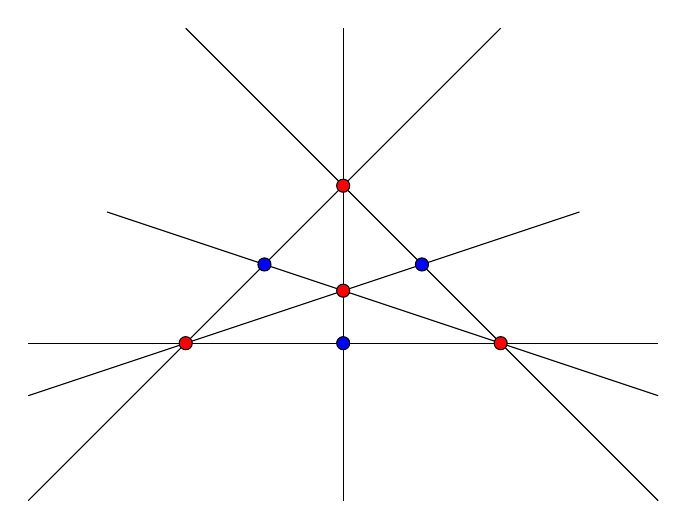
\begin{tikzpicture}
				%lines
				\draw (-4,0) to (4,0);
				\draw (-4,-2) to (2,4);
				\draw (4,-2) to (-2,4);
				\draw (0, -2) to (0,4);
				\draw (-4,-2/3) to (3,5/3);	
				\draw (4,-2/3) to (-3,5/3);
				
				%nodes
				\draw (-2,0) node [shape=circle,draw, fill=red, scale=.5] (asd) {};
				\draw (2,0) node [shape=circle,draw, fill=red, scale=.5] (asd) {};
				\draw (0,2/3) node [shape=circle,draw, fill=red, scale=.5] (asd) {};
				\draw (0,2) node [shape=circle,draw, fill=red, scale=.5] (asd) {};
				\draw (-1,1) node [shape=circle,draw,fill=blue,scale=.5] (asd) {};
				\draw (0,0) node [shape=circle,draw,fill=blue,scale=.5] (asd) {};
				\draw (1,1) node [shape=circle,draw,fill=blue,scale=.5] (asd) {};
				
				%labels
				%\draw  (0.4,-1.9) node (asd) [scale=.9] {\(H_{23}\)};
				%\draw  (3.4, 1.8) node (asd) [scale=.9] {\(H_{34}\)};
				%\draw  (-3.4,1.8) node (asd) [scale=.9] {\(H_{24}\)};
				%\draw  (-2,3.5) node (asd) [scale=.9] {\(H_{12}\)};
				%\draw  (2,3.5) node (asd) [scale=.9] {\(H_{13}\)};
				%\draw  (1,-.3) node (asd) [scale=.9] {\(H_{14}\)};
				%\draw  (-2.7, 2.7) node (asd) [scale=1.1, color=red] {\((\mathbf{CP}^2, \sum_{i<j} \mu_{ij} L_{ij} ) \)};
				\end{tikzpicture}
			}
		\end{center}
	\end{column}
	\begin{column}{.6\textwidth}
		\begin{itemize}
			\item Every line intersects the others at \((N/3)+1\) points
			\item Complex reflection groups  
			\item Complete quadrilateral (\(N=6\)) 
		\end{itemize}
	\end{column}
\end{columns}




\end{frame}

\section{2-cone}
\begin{frame}{Linear coordinates: the \(2\)-cone}
	\(C(2\pi\alpha)\) with metric \(dr^2 + \alpha^2 r^2 d\theta^2\) has  complex coordinate \(\mathcolorbox{yellow!60}{z = r^{1/\alpha} e^{i\theta}}\)
	\[\mathcolorbox{red!20}{\C_{\alpha}=\left( \C, |z|^{-2a}|dz|^2\right)}, \hspace{3mm} a=1-\alpha\]
	
	
	\begin{center}
		\scalebox{0.7}{	
			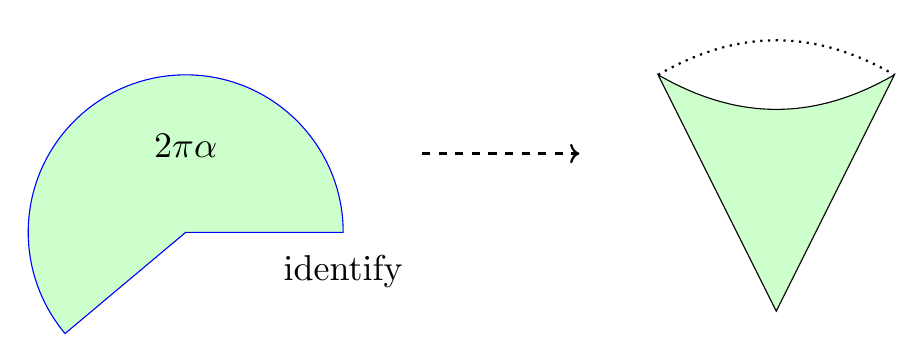
\begin{tikzpicture}
			%leftpart
			\filldraw[fill=green!20, draw=blue] (-2,0) -- (0,0) arc (0:220:2) -- (-2,0);
			\centerarc[thick](-2,0)(5:215:.7);
			\centerarc[<->,dashed,thick](-2,0)(225:355:1);
			%middle arrow
			\draw[->,dashed,thick] (1,1) to (3,1);
			%rightpart
			\filldraw[fill=green!20] (4,2) to[bend right] (7,2) -- (5.5,-1) -- cycle;
			\draw[dotted,thick] (4,2) to[bend left] (7,2);
			%nodes
			\node[scale=1.3](a) at (-2,1.1){\(2\pi\alpha\)};
			\node[scale=1.3](b) at (0,-.5){identify};
			%\node[fill=red!20,draw,rounded corners, scale=1.5](c) at (-4.5,2.5){\(0<\beta<1\)};
			\end{tikzpicture}
		}
	\end{center}
	
	\begin{itemize}
		\item Levi-Civita connection \(\nabla = d + \p \log |s|^2\) (with \(s=\p/\p z\)) is
		\[ \mathcolorbox{blue!20}{\nabla = d - a \frac{dz}{z}} \]
		\item Euler vector field \(e = (1/\alpha) \p / \p z\)
	\end{itemize}
	
\end{frame}



\section{Connection C2}

\begin{frame}{Linear coordinates on PK cones: \(\dim_{\C}=2\)}
	Regular PK cone \(\iff\) spherical metric with cone points at \(L_i \in \CP^1\)
	\textbf{Linear complex coordinates} \((z,w)\) on \(\C^2\) such that:
	\begin{itemize}
		\item \(L_i=\{\ell_i(z,w)=0\}\) complex lines through \(0\)
		\item Euler vector field is \(e=(1/\alpha_0) \left( \p / \p z + \p / \p w\right)\) %with \(2(1-\alpha_0) = \sum_{i\geq 1}(1-\alpha_i)\)  
		\item Levi-Civita connection in the \(\p/\p z, \p/\p w\) trivialization is
		\[ \nabla = d - \sum_i A_i \frac{d\ell_i}{\ell_i} \]
		where \(A_i\) are constant matrices with
		\[\tr(A_i) = a_i,  \hspace{2mm} \ker A_i = L_i, \hspace{2mm} \sum_i A_i = a_0 \cdot \Id \]
	\end{itemize}
\end{frame}

\section{stand con}
\begin{frame}{Standard connections}
	\(\mH\) finite collection of hyperplanes
	\(H \subset \C^n\) going through the origin \\
	A \textbf{standard connection} in the frame \(\p/\p z_1, \ldots, \p/ \p z_n\) has the form
	\begin{equation*}
	\mathcolorbox{blue!30}{
		\nabla = d - \sum_{\mH} A_H \frac{dh}{h}
		}
	\end{equation*}
 where \(A_H\) are non-zero constant matrices called \emph{residues}
	
	\begin{itemize}
		\item \(\nabla\) is torsion free \(\iff\) \(\mathcolorbox{green!30}{\ker A_H = H}\)
		\item \(\nabla\) is flat \(\iff\) \(\mathcolorbox{green!30}{[A_L, A_H] = 0}\) \(\forall L \subset H\) (enough \(\codim L=2\))
	\end{itemize}
\[\text{Notation: } A_L = \sum_{H|L \subset H} A_H, \hspace{2mm} A_H(v) = dh(v) \cdot n_H \]

\textbf{Obstruction:} \(H' \pitchfork H\) implies \([A_H, A_{H'}]=0\) hence \(\C \cdot n_H \subset H'\)
\end{frame}

\section{Lau}
\begin{frame}{Example: Lauricella connection \(\nabla^a\)}
	\begin{columns}
		\begin{column}{.7\textwidth}
			\begin{itemize}
				\item Braid arrangement \(H_{ij}=\{z_i=z_j\} \subset \C^{n+1}\) 
				\item \(a=(a_1, \ldots, a_{n+1}) \in \C^{n+1}\) parameters 
				\item Jordan-Pochammer matrices 
				\(A_{ij}(\vec{\mathbf{v}}) = (v_i-v_j)(a_j \vec{\mathbf{e}}_i- a_i \vec{\mathbf{e}}_j)\)
				\item Quotient by main diagonal \(\C \cdot (1, \ldots, 1)\)
			\end{itemize}
		\end{column}
	
		\begin{column}{.4\textwidth}
				\begin{figure}
				\scalebox{.4}{
					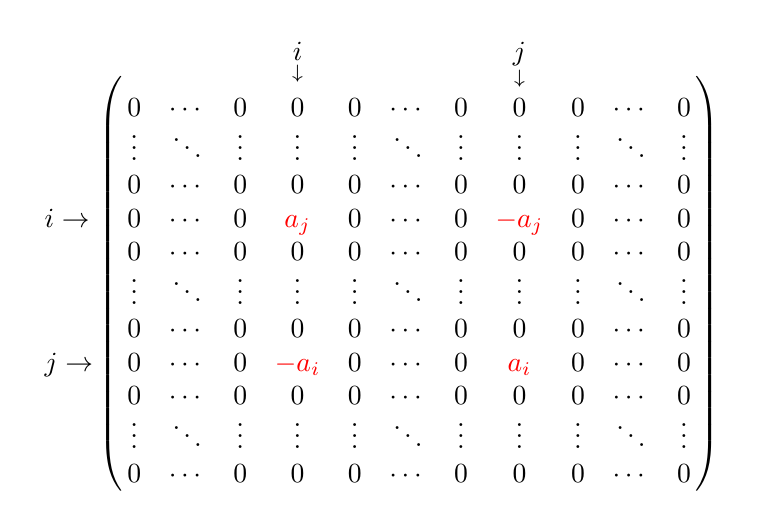
\begin{tikzpicture}
					\node at (0,0){\(\bordermatrix{ 
							& & & &  \underset{\downarrow}{i} &  & & & \underset{\downarrow}{j} \cr 
							& 0 & \cdots & 0 & 0 & 0 & \cdots & 0 & 0 & 0 & \cdots & 0 \cr 
							& \vdots & \ddots & \vdots & \vdots & \vdots & \ddots & \vdots & \vdots & \vdots & \ddots & \vdots \cr
							& 0 & \cdots & 0 & 0 & 0 & \cdots & 0 & 0 & 0 & \cdots & 0 \cr
							i \to & 0 & \cdots & 0 & {\color{red}a_j} & 0 & \cdots & 0 & {\color{red}-a_j} & 0 & \cdots & 0 \cr
							& 0 & \cdots & 0 & 0 & 0 & \cdots & 0 & 0 & 0 & \cdots & 0  \cr
							& \vdots & \ddots & \vdots & \vdots & \vdots & \ddots & \vdots & \vdots & \vdots & \ddots & \vdots \cr
							& 0 & \cdots & 0 & 0 & 0 & \cdots & 0 & 0 & 0 & \cdots & 0  \cr
							j \to & 0 & \cdots & 0 & {\color{red}-a_i} & 0 & \cdots & 0 & {\color{red}a_i} & 0 & \cdots & 0 \cr
							& 0 & \cdots & 0 & 0 & 0 & \cdots & 0 & 0 & 0 & \cdots & 0  \cr
							& \vdots & \ddots & \vdots & \vdots & \vdots & \ddots & \vdots & \vdots & \vdots & \ddots & \vdots \cr
							& 0 & \cdots & 0 & 0 & 0 & \cdots & 0 & 0 & 0 & \cdots & 0
						} \)};
					\end{tikzpicture}		
					
				}
			\end{figure}
		\end{column}
	\end{columns}
	
	\[\mathcolorbox{blue!30}{
	\nabla^a = d - \sum_{i<j} A_{ij} \frac{d(z_i-z_j)}{z_i-z_j}
	} 
	\]
	\begin{itemize}
		\item \(\ker A_{ij} = H_{ij}\) and \(\tr(A_{ij})=a_i + a_j\)
		\item \([A_{ij}, A_{kl}]=0\) if \(\{i,j\}\cap\{k,l\}=\emptyset\) and \([A_{ij}, A_{ik}+A_{jk}]\) if \(i<j<k\)
		\item (\(n=2\)) \(3\) lines in \(\C^2\) and (\(n=3\)) \(6\) planes in \(\C^3\)  (complete quad.)
	\end{itemize}
\end{frame}






\section{Main}


\begin{frame}{Main result}
\(\nabla\) standard flat torsion free \textbf{unitary} connection
i.e. \(\mbox{Hol}(\nabla) \subset U(n)\)

	\begin{itemize}
		\item Non-integer: \(a_H = \tr A_H \in \R \setminus \mathbf{Z}\) 
		
		\item Positivity: \(a_L = (\codim L)^{-1} \sum_{L \subset H} a_H < 1\) (i.e. \(\alpha_L=1-a_L>0\))
	\end{itemize}

	\begin{theorem}[dB-Panov, 2021]
		The metric completion is a polyhedral K\"ahler cone metric on \(\C^n\) with cone angles \(2\pi\alpha_H\) along \(H\)
	\end{theorem}

\begin{itemize}
	\item We allow \(\alpha_H>1\)
	\item Quotient by \(\C^*\) polyhedral Fubini-Study metrics 
	\item The volume form of the PK cone is
	\(\left(\prod |h|^{-2a_H}\right) dz \wedge d \bar{z}\) 
	\item Positivity \(\iff \prod |h|^{-2a_H}\) is locally integrable
\end{itemize}

\end{frame}


\section{Application}

\begin{frame}{Application: the braid arrangement}
	Recall the (essential) braid arrangement is made of \(\binom{n+1}{2}\) hyperplanes 
	\[
	H_{ij}=\{z_i=z_j\} \subset  \C^{n+1} / \C \cdot (1, \ldots, 1)
	\]
	For each \(a=(a_1, \ldots, a_{n+1})\) there is a \textbf{Lauricella connection} \(\nabla^a\)
	\begin{itemize}
		\item If \(a \in \R^{n+1}\) and \(\{a_i\} \neq 0\) for all \(i\) then \(\nabla^a\) admits a (unique up to scale) non-degenerate invariant Hermitian form
		\item The signature is \((p, n-p)\) with
		\[p =  \lfloor \sum_{i=1}^{n+1} \{a_i\} \rfloor \tag{Deligne-Mostow}  \]
	\end{itemize}
	
	
	
	\begin{columns}
		\begin{column}{0.38\textwidth}
			\begin{itemize}
				\item 	\(n=2 \to\) sphere with three cone points
			\end{itemize}
			
			
		\end{column}
		\begin{column}{.48\textwidth}
			\begin{center}
				\begin{figure}
					\includegraphics[width=0.6\textwidth,height=0.6\textheight,keepaspectratio]{HOLES1}
				\end{figure}
			\end{center}
		\end{column}		
	\end{columns}
\end{frame}

\section{Proof}

\begin{frame}{Proof}
	\begin{enumerate}
		\item Induction on \(n\). For \(n=1\) we have \(\nabla=d-adz/z\) and positivity \(\alpha=1-a>0\) is all we need
		\item Enough to show \emph{local product decomposition} away from the origin (characterization of polyhedral metrics by Lebedeva-Petrunin)
		\item Close to \(x \in L\) write  \(\nabla = \nabla^L + \mbox{(hol.)}\) with \(\nabla^L\) standard and splits according to the product decomposition of \(\mH_L=\{H \in \mH| L \subset H\}\)
		\item Holomorphic frame \(G: U \setminus \mH \to GL(n, \C)\) such that \(G^*\nabla^L=\nabla\) (semi-simple representations have closed conjugate orbits)
		\item \(G\) extends holomorphically over \(\mH\) (non-integer condition, normal form for logarithmic connections)
		\item \textbf{Local dilation vector field} \(e_x = e_0 - s\) where \(s\) is a parallel vector field \(\nabla s = 0\) with \(s(x)=e_0(x)\) (constructed using \(G\))
		\item Linearise \(e_x\) (Poincar\'e-Dulac)
	\end{enumerate}
\centering
{\color{blue}{\huge{\textbf{THANK YOU!}}}}
\end{frame}



\end{document}
